\newpage
\section{Aufgabe 1}
	In der abgebildeten Schaltung sollen Strom und Spannung gemessen werden.\\
	\subsection{Aufgabe 1a}
		Erläutern Sie kurz die Begriffe Strom und Spannung und zeichnen Sie in der Schaltung die korrekte Position von Volt- und Amperemeter ein.\\
		\textbf{Strom}\\
		Der elektrische Strom oder elektrische Stromstärke wird kurz Strom genannt. Damit ist die Übertragung elektrischer Energie gemeint. Der elektrische Strom ist die gezielte und gerichtete Bewegung freier Ladungsträger. Die Ladungsträger können Elektronen oder Ionen sein.\\ \\
		\textbf{Spannung}\\
		Die elektrische Spannung U gibt die Differenz der Ladungen zwischen zwei Polen an. Spannungsquellen besitzen immer zwei Pole mit unterschiedlichen Ladungen. Am Pluspol ist ein Mangel an Elektronen. Und am Minuspol ist ein Überschuss an Elektronen. Diese Differenz der Elektronenmenge nennt man elektrische Spannung. Entsteht eine Verbindung zwischen den Polen, kommt es zu einer Entladung. Bei diesem Vorgang flie\ss{}t ein elektrischer Strom.\\ \\
		\begin{figure}[h]
			\centering
			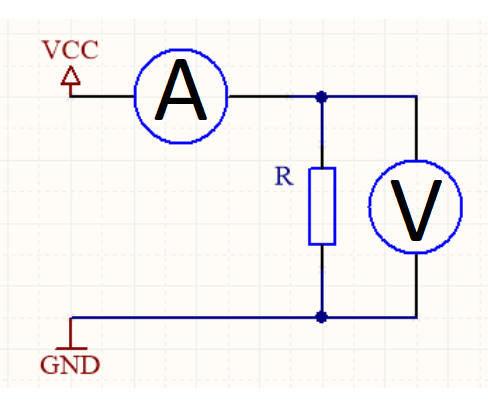
\includegraphics[width=0.7\linewidth]{images/Strom_Spannung}
			\caption{}
			\label{fig:Strom_Spannung}
		\end{figure}
	\subsection{Aufgabe 1b}
		Sie haben eine Gleichspannung von 12V und eine Stromstärke von 500$\mu$A gemessen. Wie gro\ss{} ist der Widerstand des Verbrauchers R?\\
		$
		U = 12V, I = 500\mu A = 0,5mA = 0,0005A\\
		R = \frac{U}{I}\\
		R = \frac{12V}{0,0005A}\\
		R = 24000\Omega = 24k\Omega\\
		$
		Der Widerstand des Verbrauchers R beträgt 24k$\Omega$.\\
	\subsection{Aufgabe 1c}
		Mit welcher maximalen Stromstärke darf ein 1M$\Omega$ Widerstand betrieben werden, dessen Nennleistung 0,33W beträgt?\\
		$
		R = 1M\Omega = 1000k\Omega = 1000000\Omega, P = 0,33W\\
		P = U * I, U = R * I\\
		P = R * I^{2}\\
		I^{2} = \frac{P}{R}\\
		I = \sqrt{\frac{P}{R}}\\
		I = \sqrt{\dfrac{0,33W}{1000000\Omega}}	\\
		I = \sqrt{\dfrac{0,00000033* V * A}{\frac{V}{A}}}\\
		I = \sqrt{0,00000033* A^{2}}\\
		I = 0,000574456A = 0,574456mA = 574,456\mu A\\
		$
		Ein 1M$\Omega$ Widerstand mit einer Nennleistung von 0.33W darf mit maximal 574,456$\mu$A betrieben werden.\\
\newpage
\section{Aufgabe 2}
	\begin{figure}[h]
		\centering
		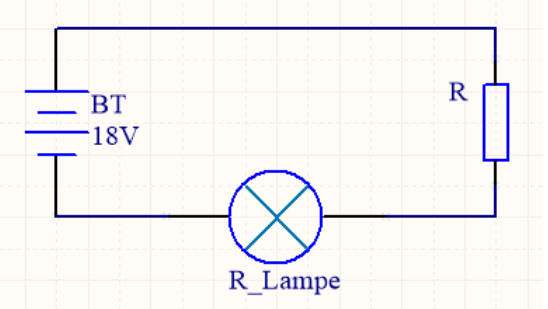
\includegraphics[width=0.5\linewidth]{images/Stromkreis_Lampe}
		\caption{}
		\label{fig:Stromkreis_Lampe}
	\end{figure}
	Aus dem Datenblatt der Batterie:\\
	\begin{itemize}
		\item Nennspannung: 18V, Kapazität: 90Ah\\
	\end{itemize}
	Aus dem Datenblatt der Lampe:\\
	\begin{itemize}
		\item Betriebsspannung: 12V AC/DC\\
		\item Leistung: 60 Watt\\
	\end{itemize}
	\subsection{Aufgabe 2a}
		Welche maximale Stromstärke ist bei 12V nötig, damit die Lampe eine Leistung von 60 Watt umsetzt?\\
		$
		U = 12V, P = 60W\\
		P = U * I\\
		I = \frac{P}{U}\\
		I = \frac{60W}{12V} = \frac{60 * V * A}{12V}\\
		I = 5A\\
		$
		Bei 12V werden 5A benötigt damit die Lampe eine Leistung von 60 Watt umsetzt.\\
	\subsection{Aufgabe 2b}
		Kann der Verbraucher $R_{Lampe}$ direkt an der Spannungsquelle betrieben werden? Begründung! Sollten Sie einen Widerstand R benötigen, Begründung und Widerstand in $\Omega$ angeben.\\
		$ 
		U = 18V, I = 5A, U_{Lampe} = 12V\\
		U_{R} = U - U_{Lampe}\\
		U_{R} = 18V - 12V = 6V\\
		R = \frac{U_{R}}{I}\\
		R = \frac{6V}{5A}\\
		R = 1,2\Omega\\
		$
		Der Verbraucher $R_{Lampe}$ darf nicht direkt an der Spannungsquelle betrieben werden, da die Nennspannung der Batterie grö\ss{}er als die Betriebsspannung der Lampe ist. Es wird ein Widerstand R mit 1,2$\Omega$ benötigt. Der Widerstand R teilt die Spannung in 6V und 12V.\\
	\subsection{Aufgabe 2c}
		Wie lange kann Ihre Schaltung betrieben Werden, bis die Batterie erschöpft ist?\\
		$ 
		Q = 90Ah, U = 18V, I = 5A, P_{Lampe} = 60W, U_{R} = 6V\\
		P_{R} = U_{R} * I\\
		P_{R} = 6V * 5A = 30W\\
		P = P_{R} + P_{Lampe}\\
		P = 30W + 60W = 90W\\
		W = Q * U\\
		W = 90Ah * 18V = 1620VAh = 1620Wh\\
		P = \frac{W}{t}\\
		W = P * t\\
		t = \frac{W}{P}\\
		t = \frac{1620Wh}{90W} = 18h\\
		$
		Die Schaltung kann 18 Stunden betrieben werden.\\
\newpage
\section{Aufgabe 3}
	Verschaffen Sie sich einen Überblick, identifizieren Sie die Bauteile und erläutern Sie kurz die Funktion der abgebildeten Schaltung.\\
	\begin{figure}[h]
		\centering
		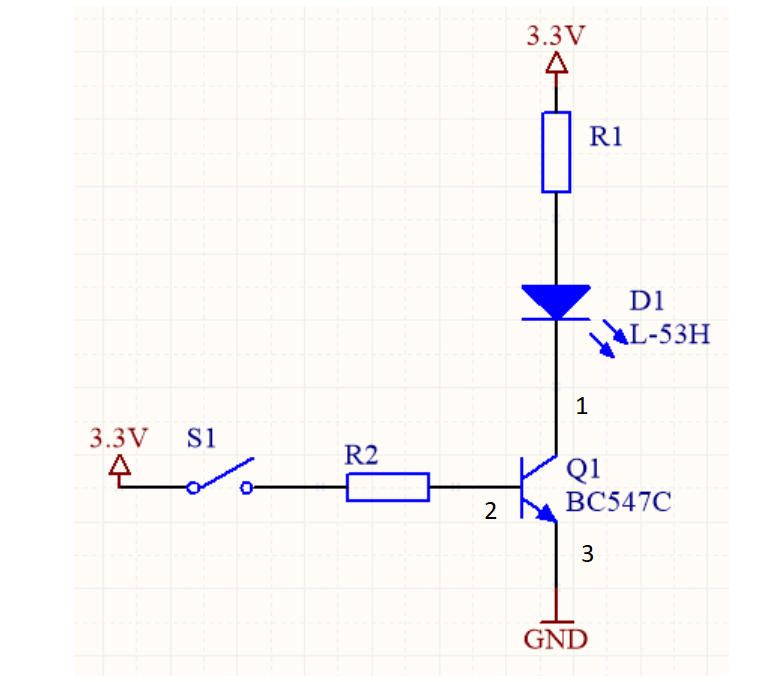
\includegraphics[width=0.4\linewidth]{images/Transistor_Schaltung}
		\caption{}
		\label{fig:Transistor_Schaltung}
	\end{figure}
	\\Gegeben: \\
	$V_{CC}$ +3,3V\\
	$Q_{1}$ BC547C (Datenblatt unter \url{https://www.fairchildsemi.com/datasheets/BC/BC547.pdf})\\
	$D_{1}$ Kingbright L-53H (Datenblatt unter \url{https://cdn-reichelt.de/documents/datenblatt/A500/LED5MMSTGE\_LED5MMSTGN\_LED5MMSTRT\%23KIN.pdf})\\	
	$R_{2} 4.2 k\Omega$\\
	\subsection{Aufgabe 3a}
		Entnehmen Sie aus dem Datenblatt die Spannung und Stromstärke für den Regelbetrieb der LED $D_{1}$.\\
		$
		I_{D1} = 20mA, U_{D1} = 2,0V, U_{D1Max} = 2,5V (In Durchlassrichtung)\\
		I_{D1} = 10\mu A, U_{D1} = 5,0V (In SperrrichtunG)\\
		$
	\subsection{Aufgabe 3b}
		Suchen Sie im Datenblatt des Transistors nach der Pinbelegung für Collector, Emitter und Base.\\
		Pin 1. Collector\\
		Pin 2. Base\\
		Pin 3. Emitter\\
	\subsection{Aufgabe 3c}
		Berechnen Sie den Vorwiderstand $R_{1}$ genau und runden Sie den Widerstandswert für den Aufbau sinnvoll. Am Transistor $Q_{1}$ gibt es einen Spannungsabfall, den Sie hier mit 640mV annehmen können. Bauen Sie die Schaltung auf, lassen Sie sich die Schaltung vom Betreuer VOR dem Einschalten abnehmen und überprüfen Sie die Funktionsweise.\\
		$
		U = 3,3V, I_{R1} = 20mA = 0,02A, U_{T} = 640mV = 0,64V, U_{LED} = 2,5V\\
		U_{R1} = U - U_{LED} - U_{T}\\
		U_{R1} = 3,3V - 2,5V - 0,64V\\
		U_{R1} = 0,16V\\
		R_{1} = \frac{U_{R1}}{I_{R1}}\\
		R_{1} = \frac{0,16V}{0,02A}\\
		R_{1} = 8\Omega\\
		$
		Der Vorwiderstand beträgt gerundet 10$\Omega$.\\
\section{Quellen}
	\begin{quote}
		\begin{itemize}
			\item \url{https://www.elektronik-kompendium.de/sites/grd/0110203.htm} \\Zugriff: 06.05.2018\\
			\item \url{https://www.elektronik-kompendium.de/sites/grd/0201101.htm} \\Zugriff: 06.05.2018\\
			\item \url{https://www.elektronik-kompendium.de/sites/bau/0201111.htm} \\Zugriff: 06.05.2018\\
			\item \url{https://www.elektronik-kompendium.de/sites/bau/0201291.htm} \\Zugriff: 06.05.2018\\
			\item \url{https://www.elektronik-kompendium.de/sites/slt/0203111.htm} \\Zugriff: 06.05.2018\\
		\end{itemize}
	\end{quote}